\documentclass[../thesis.tex]{subfiles}
\begin{document}

\chapter{Background}
\label{chap:back}

The following chapter presents a thorough treatment of the literature on the application of ML techniques for the assessment of heart failure\footnote{We highly recommend reading \cite{tripoliti2017heart} for a broader overview of the literature on the state-of-the-art ML techniques applied for the assessment of heart failure.}. Important topics such as HF detection, subtype estimation and prediction of clinical outcomes in the context of ML will be presented and explained.

\section{HF detection}
\label{sec:hfdet}

\noindent The ESC defines HF as a clinical syndrome caused by structural and/or functional cardiac abnormality, resulting in a reduced cardiac output (CO) and/or elevated intracardiac pressures at rest or during stress. It is typically characterized by symptoms, such as breathlessness, ankle swelling and fatigue that may be accompanied by signs, such as elevated jugular venous pressure (JVP), pulmonary crackles and peripheral oedema (swelling in lower limbs) \citep{ponikowski2016}. HF prevents the heart from fulfilling the circulatory demands from the body, due to its impairing abilities on the ventricles to maintain the bodies hemodynamics (blood flow). As there is no broad definitive industry accepted diagnostic test for HF, one finds in clinical practice that medical diagnosis is done with a combination of careful examinations (physical and historical) with assisting tests, such as blood tests, chest radiography (chest X-ray, CXR), electrocardiography (EKG) and echocardiography (cardiac echo), see e.g \cite{henein2010heart} and \cite{son2012decision}. As a result of this, several criteria for determining the presence of HF have been proposed, including the Framingham criteria \citep{mckee1971natural}, the Boston criteria \citep{carlson1985analysis}, the Gothenburg criteria \citep{eriksson1987cardiac} and the ESC criteria \citep{swedberg2005guidelines} \citep{roger2010heart}. All of which are widely used in clinical practise.\\
\indent In a non-acute onset, the ESC has also defined an algorithm for diagnosing HF \citep{ponikowski2016}. The algorithm is structured in the following way: First, the probability of HF ($\hat{p}_{HF}$) is evaluated along three dimensions: 
\begin{enumerate}[label=(\roman*)]
    \item \textbf{Prior clinical history}: History of coronary artery disease (CAD) or arterial hypertension, exposition to cardiotoxic drugs/ radiation, diuretic use (any substance that promotes the production of urine) or orthopnea (shortness of breath when lying down)
    \item \textbf{Physical examination}: Crackles/rales, bilateral ankle oedema (swelling in both ankles), abnormal heart sounds/murmur, jugular venous dilatation, laterally displaced/broadened apical beat (pulse felt at the point of maximum impulse (PMI))
    \item \textbf{Abnormalities in electrocardiography (EKG)}
\end{enumerate}
\indent If all elements along the three dimensions are normal/absent, $\hat{p}_{HF}$ is estimated to be highly unlikely. If at least one element is abnormal, then plasma Natriuretic Peptides (NP)\footnote{A hormone, mainly secreted from the heart, that has important natriuretic and kaliuretic properties (excretion of sodium and potassium in the urine) \citep{pandit2011natriuretic}. In clinical practice it is found that brain NP (also called BNP) levels can be used to predict the risk of death and cardiovascular events  \citep{wang2004plasma}.} should be measured in order to identify patients who need echocardiography. Specifically, if the NP values are above the exclusion threshold\footnote{The recommended threshold levels are BNP levels $\geq 35 pg/mL$ or NTproBNP levels $\geq 125 pg/mL$, see e.g. \cite{cowie1997value}, \cite{yamamoto2000clinical}, \cite{krishnaswamy2001utility}, \cite{zaphiriou2005diagnostic}, \cite{fuat2006diagnostic} and \cite{maisel2008state}.} or should the assessment of NPs not be routinely done in clinical practice then patients need to be forwarded for an echocardiography. With the help of the cardiac echo, specialists can detect abnormalities in the heart rhythm. Should the results of the plasma NP or the echocardiography be normal\footnote{Normal ventricular and atrial volumes and function \citep{aune2009normal}.}, then HF is also considered unlikely. \begin{figure}

\centering



\tikzset{every picture/.style={line width=0.75pt}} %set default line width to 0.75pt        

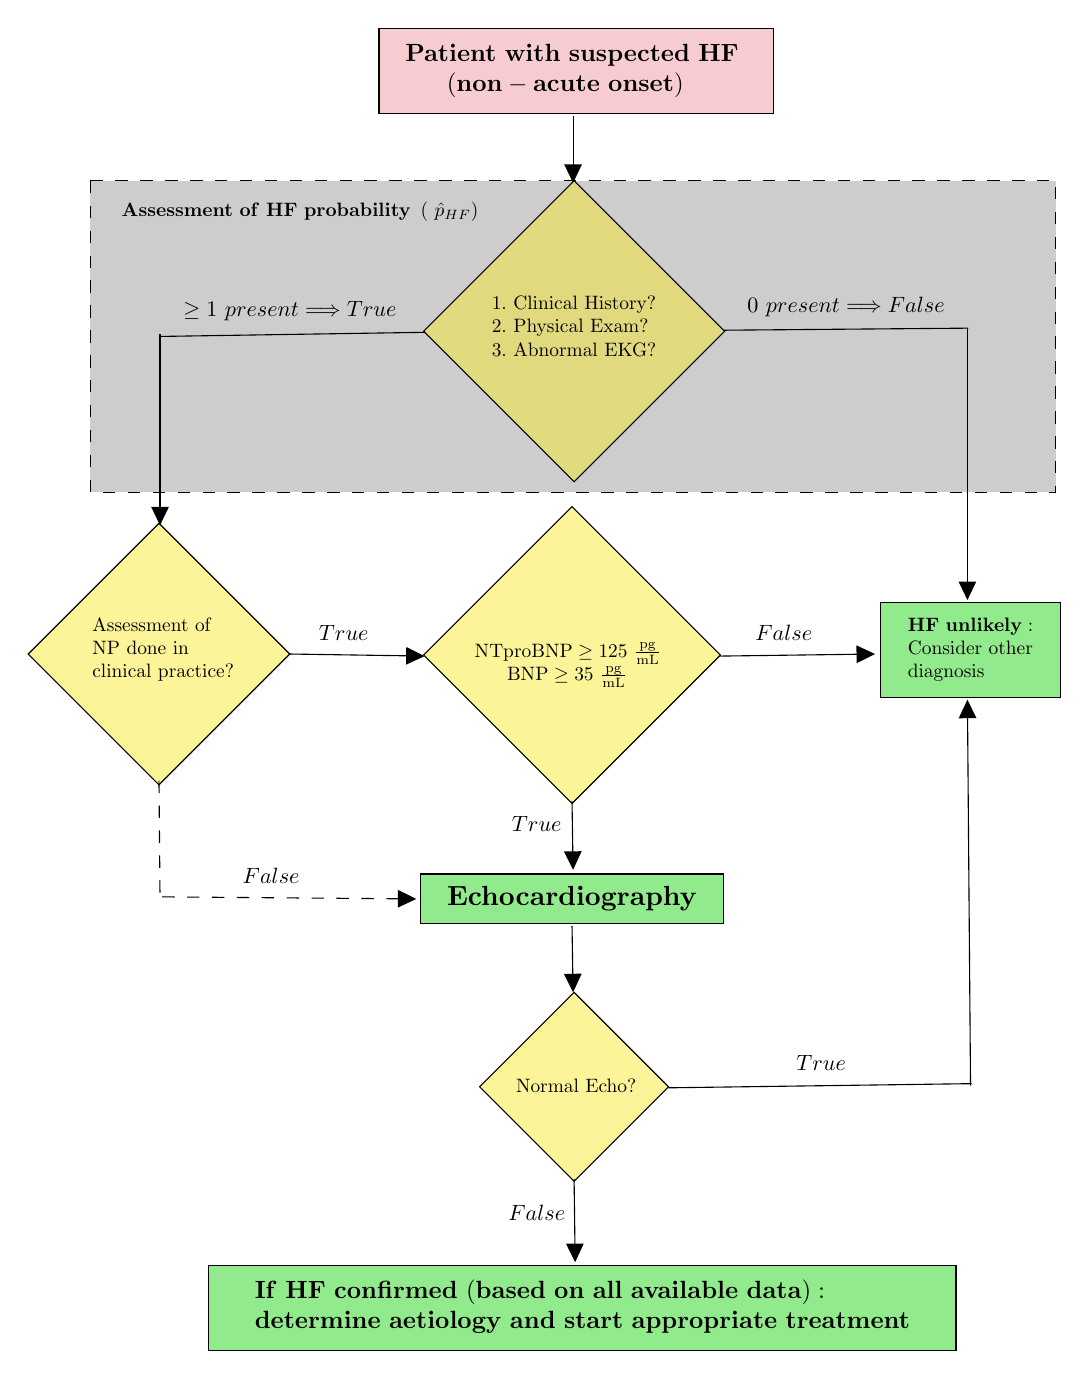
\begin{tikzpicture}[x=0.75pt,y=0.75pt,yscale=-1,xscale=1]
%uncomment if require: \path (0,652); %set diagram left start at 0, and has height of 652

%Shape: Rectangle [id:dp05338957976791869] 
\draw  [fill={rgb, 255:red, 155; green, 155; blue, 155 }  ,fill opacity=0.5 ][dash pattern={on 4.5pt off 4.5pt}] (35,80) -- (500,80) -- (500,230) -- (35,230) -- cycle ;
%Straight Lines [id:da055858825280932] 
\draw    (267.5,49) -- (267.5,79) ;
\draw [shift={(267.5,81)}, rotate = 270] [fill={rgb, 255:red, 0; green, 0; blue, 0 }  ][line width=0.75]  [draw opacity=0] (8.93,-4.29) -- (0,0) -- (8.93,4.29) -- cycle    ;

%Straight Lines [id:da4365110914453669] 
\draw    (68.5,155) -- (196.5,153) ;


%Straight Lines [id:da3272244813405638] 
\draw    (68.5,154) -- (68.5,244) ;
\draw [shift={(68.5,246)}, rotate = 270] [fill={rgb, 255:red, 0; green, 0; blue, 0 }  ][line width=0.75]  [draw opacity=0] (8.93,-4.29) -- (0,0) -- (8.93,4.29) -- cycle    ;

%Straight Lines [id:da17400033500022816] 
\draw    (457.5,151) -- (457.5,280) ;
\draw [shift={(457.5,282)}, rotate = 270] [fill={rgb, 255:red, 0; green, 0; blue, 0 }  ][line width=0.75]  [draw opacity=0] (8.93,-4.29) -- (0,0) -- (8.93,4.29) -- cycle    ;

%Straight Lines [id:da3278613507085377] 
\draw    (131,308) -- (194,308.97) ;
\draw [shift={(196,309)}, rotate = 180.88] [fill={rgb, 255:red, 0; green, 0; blue, 0 }  ][line width=0.75]  [draw opacity=0] (8.93,-4.29) -- (0,0) -- (8.93,4.29) -- cycle    ;

%Shape: Square [id:dp3364304080096274] 
\draw  [fill={rgb, 255:red, 248; green, 231; blue, 28 }  ,fill opacity=0.45 ] (268,80) -- (340.5,152.5) -- (268,225) -- (195.5,152.5) -- cycle ;
%Straight Lines [id:da1685251091101021] 
\draw    (340,152) -- (458,151) ;


%Straight Lines [id:da2968793712930289] 
\draw    (338.5,309) -- (411,308.03) ;
\draw [shift={(413,308)}, rotate = 539.23] [fill={rgb, 255:red, 0; green, 0; blue, 0 }  ][line width=0.75]  [draw opacity=0] (8.93,-4.29) -- (0,0) -- (8.93,4.29) -- cycle    ;

%Straight Lines [id:da5449359734131121] 
\draw  [dash pattern={on 4.5pt off 4.5pt}]  (69.5,425) -- (190,425.98) ;
\draw [shift={(192,426)}, rotate = 180.47] [fill={rgb, 255:red, 0; green, 0; blue, 0 }  ][line width=0.75]  [draw opacity=0] (8.93,-4.29) -- (0,0) -- (8.93,4.29) -- cycle    ;

%Straight Lines [id:da5016779396235063] 
\draw  [dash pattern={on 4.5pt off 4.5pt}]  (68,369) -- (68.5,426) ;


%Straight Lines [id:da7236757292406453] 
\draw    (267,439) -- (267.47,469) ;
\draw [shift={(267.5,471)}, rotate = 269.1] [fill={rgb, 255:red, 0; green, 0; blue, 0 }  ][line width=0.75]  [draw opacity=0] (8.93,-4.29) -- (0,0) -- (8.93,4.29) -- cycle    ;

%Straight Lines [id:da760594202182669] 
\draw    (313.5,517) -- (459.5,515) ;


%Straight Lines [id:da3750532871622436] 
\draw    (459,516) -- (457.52,332) ;
\draw [shift={(457.5,330)}, rotate = 449.54] [fill={rgb, 255:red, 0; green, 0; blue, 0 }  ][line width=0.75]  [draw opacity=0] (8.93,-4.29) -- (0,0) -- (8.93,4.29) -- cycle    ;

%Shape: Square [id:dp7874754730652669] 
\draw  [fill={rgb, 255:red, 248; green, 231; blue, 28 }  ,fill opacity=0.45 ] (267,237) -- (338.5,308.5) -- (267,380) -- (195.5,308.5) -- cycle ;
%Shape: Square [id:dp19176781264401277] 
\draw  [fill={rgb, 255:red, 248; green, 231; blue, 28 }  ,fill opacity=0.45 ] (68,245) -- (131,308) -- (68,371) -- (5,308) -- cycle ;
%Shape: Square [id:dp8240263825354897] 
\draw  [fill={rgb, 255:red, 248; green, 231; blue, 28 }  ,fill opacity=0.45 ] (268,471) -- (313.5,516.5) -- (268,562) -- (222.5,516.5) -- cycle ;
%Straight Lines [id:da9916785343630015] 
\draw    (267,379) -- (267.47,410) ;
\draw [shift={(267.5,412)}, rotate = 269.13] [fill={rgb, 255:red, 0; green, 0; blue, 0 }  ][line width=0.75]  [draw opacity=0] (8.93,-4.29) -- (0,0) -- (8.93,4.29) -- cycle    ;

%Straight Lines [id:da8876972127593497] 
\draw    (268,561) -- (268.48,599) ;
\draw [shift={(268.5,601)}, rotate = 269.28] [fill={rgb, 255:red, 0; green, 0; blue, 0 }  ][line width=0.75]  [draw opacity=0] (8.93,-4.29) -- (0,0) -- (8.93,4.29) -- cycle    ;


% Text Node
\draw  [fill={rgb, 255:red, 139; green, 233; blue, 134 }  ,fill opacity=0.95 ]  (194,414) -- (340,414) -- (340,438) -- (194,438) -- cycle  ;
\draw (267,426) node [scale=1]  {$\mathbf{Echocardiography}$};
% Text Node
\draw  [fill={rgb, 255:red, 139; green, 233; blue, 134 }  ,fill opacity=0.95 ]  (415.5,283) -- (502.5,283) -- (502.5,329) -- (415.5,329) -- cycle  ;
\draw (459,306) node [scale=0.7]  {$ \begin{array}{l}
\mathbf{HF\ unlikely:}\\
\mathrm{Consider\ other}\\
\mathrm{diagnosis}
\end{array}$};
% Text Node
\draw (157,298) node [scale=0.8]  {$True$};
% Text Node
\draw (369,298) node [scale=0.8]  {$False$};
% Text Node
\draw (250,390) node [scale=0.8]  {$True$};
% Text Node
\draw (122,415) node [scale=0.8]  {$False$};
% Text Node
\draw (136,95) node [scale=0.7]  {$\mathbf{Assessment\ of\ HF\ probability} \ \left( \ \hat{p}_{HF}\right)$};
% Text Node
\draw (387,505) node [scale=0.8]  {$True$};
% Text Node
\draw (250,577) node [scale=0.8]  {$False$};
% Text Node
\draw (268,151) node [scale=0.7]  {$ \begin{array}{l}
\mathrm{1.\ Clinical\ History?}\\
\mathrm{2.\ Physical\ Exam?}\\
\mathrm{3.\ Abnormal\ EKG?}
\end{array}$};
% Text Node
\draw (131,143) node [scale=0.8]  {$\geq 1\ present\Longrightarrow True$};
% Text Node
\draw (399,141) node [scale=0.8]  {$0\ present\Longrightarrow False$};
% Text Node
\draw (70,306) node [scale=0.7]  {$ \begin{array}{l}
\mathrm{Assessment\ of\ }\\
\mathrm{NP\ done\ in\ }\\
\mathrm{clinical\ practice?}
\end{array}$};
% Text Node
\draw (265,313) node [scale=0.7]  {$ \begin{array}{l}
\mathrm{NTproBNP\geq 125\ \frac{pg}{mL}}\\
\mathrm{\ \ \ \ \ BNP\geq 35\ \frac{pg}{mL}}
\end{array}$};
% Text Node
\draw  [fill={rgb, 255:red, 139; green, 233; blue, 134 }  ,fill opacity=0.95 ]  (92,602.5) -- (452,602.5) -- (452,643.5) -- (92,643.5) -- cycle  ;
\draw (272,623) node [scale=0.9]  {$ \begin{array}{l}
\mathbf{If\ HF\ confirmed\ ( based\ on\ all\ available\ data) :}\\
\mathbf{determine\ aetiology\ and\ start\ appropriate\ treatment}
\end{array}$};
% Text Node
\draw (269,516) node [scale=0.7]  {$\mathrm{Normal\ Echo?}$};
% Text Node
\draw  [fill={rgb, 255:red, 208; green, 2; blue, 27 }  ,fill opacity=0.2 ]  (174,6.5) -- (364,6.5) -- (364,47.5) -- (174,47.5) -- cycle  ;
\draw (269,27) node [scale=0.9]  {$ \begin{array}{l}
\mathbf{Patient\ with\ suspected\ HF\ }\\
\mathbf{\ \ \ \ \ ( non-acute\ onset)}
\end{array}$};


\end{tikzpicture}

\caption[ESC diagnostic algorithm of heart failure]{\textit{ESC diagnostic algorithm for the diagnosis of heart failure of non-acute onset \cite[page.~2141]{ponikowski2016}.}}
\label{fig:esc_algo_hf}
\normalsize
\end{figure} Should the results of the echo yield any abnormal results, appropriate HF treatment should be initiated. The structure of the ESC algorithm is illustrated in the flow chart in Figure (\ref{fig:esc_algo_hf}). Being that the ESC algorithm is much used in clinical practice throughout the world, there is research that suggest that the medical and economic benefits of applying ML in the detection of HF should not be ignored. In the context of diagnosing patients with HF, the benefits typically include: (i) less time consumption, (ii) more support (large global community of ML practitioners in business and academia) and (iii) same level of accuracy as conventional tools when applied on available data. Many ML methods used to detect HF as a statistical learning problem, fall in the category of \textit{supervised} statistical learning (see section \ref{subsec:supervisedlearn}). The relevant ones include expressing the detection of HF as a two class classification problem, where the presence of HF is the output of the classifiers. Methods including logistic regression, linear discriminant analysis (LDA), Bayesian classifier, k-nearest neighbours (k-NN), random forests (RF), boosting, support vector machines (SVM) and neural networks (NN) are all very popular. As the response variable of the classification problem is categorical, most ML studies tend to use measures of heart rate variability (HRV)\footnote{HRV is the amount of heart rate fluctuations around the mean heart rate \citep{van1993heart}. The HRV can be assessed using R-waves produced by an EKG and reduced HRV is typically an established sign of HF \citep{ernst2016heart}.} as the main predictors for distinguishing patients as normal or with HF \citep{tripoliti2017heart}. Other predictors include parameters from clinical tests (i.e. blood test, echo, EKG, chest radiography), clinical variables (e.g. gender, age, blood pressure, smoking habit) and other lab-


\begin{footnotesize}
\begin{tabularx}{\textwidth}{Lp{1cm}LLLp{3cm}}
\caption{Literature review of HF detection}\\
\toprule
Author & HRV? & Method & Data & Features & Evaluation\\
\midrule
\endfirsthead
\caption*{\textbf{Table \ref{tab:ML_HF_detection_lit}:} Literature review of HF detection (\textit{continued})} \label{tab:ML_HF_detection_lit}\\
\toprule
Author & HRV? & Method & Data & Features & Evaluation\\
\midrule
\endhead
\cite{masetic2016congestive} & False & SVM, k-NN, NN, RF & $N = 28$ (13 normal and 15 HF) & Response: Normal \& HF. Predictor: Features extracted by EKG. & SVM:\newline Accuracy: 99.53\%\newline k-NN:\newline Accuracy: 99.93\%\newline NN:\newline Accuracy: 99.20\%\newline RF:\newline Accuracy: 100.00\%\newline\newline Validation: 10-fold cross validation\\
\cite{liu2014new} & True & SVM, k-NN & $N = 47$ (30 normal and 17 HF) & Response: Normal \& HF. Predictor: Short term HRV measure (ST-HRV) & SVM:\newline Accuracy: 100.00\%\newline \newline Validation: Cross-validation\\
&\\
\cite{narin2014investigating} & True & SVM, k-NN, LDA, NN & $N = 83$ (54 normal and 29 HF) & Response: Normal \& HF. Predictor: ST-HRV & SVM:\newline Accuracy: 91.56\%\newline k-NN:\newline Accuracy: 85.54\%\newline LDA:\newline Accuracy: 85.54\%\newline NN:\newline Accuracy: 89.15\%\newline \newline Validation: Leave-one-ut cross valid- ation.\\
&\\
\cite{gharehchopogh2011neural} & False & NN & $N = 40$ (26 normal and 14 HF) & Response: Normal \& HF. Predictor: Gender, age, blood pressure, smoking habits. & NN:\newline Accuracy: 95.00\%\newline \newline Validation: Testing set.\\
&\\
\cite{yang2010heart} & False & Naive-Bayes, SVM, NNC & $N=153$ (58 Nor- mal, 30 HF-prone, 65 HF) & Response: Non-HF group (Health or HF-prone) \& HF. Predictor: clinical test results & SVM:\newline Accuracy: 74.40\% \newline \newline Validation: Test set of $N=90$ subjects\\[-0,05cm]
\midrule
\end{tabularx}
\end{footnotesize}

\noindent oratory findings. Relevant articles where one applies ML techniques to address the statistical learning problem of detecting patients with HF is shown in table (\ref{tab:ML_HF_detection_lit}). Some common evaluation measures used in such research include: sensitivity (true positive rate), specificity (true negative rate), accuracy\footnote{The fraction/proportion of true positives (\textit{sensitivity}) or true negatives (\textit{specificity}) correctly identified \citep{james2013introduction}.} and Cohen's Kappa $\kappa$ \citep{cohen1960coefficient}. The accuracy is the only evaluation measure reported in Table (\ref{tab:ML_HF_detection_lit}). We also need to emphasize that as this particular statistical learning problem (i.e. detection of HF) is outside of the scope of the problem statement mentioned in chapter (\ref{chap:intro}), we will not be pursuing a further literature review of this problem. However, we highly recommend reading the likes of \cite{tripoliti2017heart}, \cite{acharya2017application} or \cite{awan2018machine}, for a more up-to-date overview of the literature on ML used for HF detection. 


\section{Subtype estimation}
\label{sec:subtypeest}

\noindent According to the ESC algorithm (Figure \ref{fig:esc_algo_hf}), once HF is confirmed and the probability of HF is assessed and estimated to be likely, the next step is to estimate the causes (aetiology) and the subtype of HF. The main definition of HF subtypes is based on historical research. Most of the research done after the 1990s emphasize estimating the subtype of HF patients based on the measure of the left ventricle ejection fraction (LVEF). The two usual ways of obtaining the LVEF values are through an echocardiography or cardiac magnetic resonance imaging (CMR or cardiac MR) \citep{ponikowski2016}. In prior guidelines presented by the ESC, HFrEF and HFpEF were the two main subtypes of HF \citep{authors2012esc}. The ESC did however acknowledge that a gray zone existed between the two. As a result of this a new subtype was introduced, namely HFmrEF. The ESC did so in hopes of stimulating research into the underlying characteristics, pathophysiology and treatment of this group of patients \citep{ponikowski2016}. Details about the criteria for the various HF subtypes are shown in Table (\ref{tab:HF_subtypes}). The differences between HFmrEF and HFpEF are difficult to distinguish. As mentioned, these two groups were previously classified as HFpEF. Diagnosing HFpEF is a very complex process with the diagnosis of chronic HEpEF being especially cumbersome in elderly patients with one or more additional diseases (comorbidity). With the exception of the LVEF 


\begin{footnotesize}
\begin{tabularx}{\textwidth}{LLLL}
\caption[HF subtypes based on LVEF]{HF subtypes based on LVEF \citep[page.~2137]{ponikowski2016}}\label{tab:HF_subtypes}\\
\toprule
Criteria & HFrEF & HFmrEF & HFpEF\\
\midrule
\endfirsthead
\caption*{\textbf{Table \ref{tab:HF_subtypes}:} HF subtypes based on LVEF (\textit{continued})}\\
\toprule
Criteria & HFrEF & HFmrEF & HFpEF\\
\midrule
\endhead
1 & Symptoms $\pm$ Signs & Symptoms $\pm$ Signs & Symptoms $\pm$ Signs\\ 
&\\
2 & LVEF $<$ 40\% & 40 $\leq$ LVEF $<$ 50 & 50 $\leq$ LVEF\\
&\\
3 & -- & 1. Elevated NP levels (fig \ref{fig:esc_algo_hf})
& 1. Elevated NP levels (fig \ref{fig:esc_algo_hf}) \\[0,1cm]
& & 2. At least one additional crit- eria: & 2. At least one additional crit- eria:\\[0,1cm]
& & \footnotesize a) Relevant structural heart disease\footnotemark &\footnotesize  a) Relevant structural heart disease\\[0,1cm]
& & \footnotesize  b) Diastolic dysfunction\footnotemark & \footnotesize  b) Diastolic dysfunction\\
\midrule
\end{tabularx}
\end{footnotesize}

\footnotetext[7]{\textit{Left ventricular hypertrophy} (LVH): Thickening of the heart muscle of the left ventricle of the heart and/or \textit{Left atrial enlargement} (LAE): Enlargement of the left atrium (LA) of the heart \citep{nagueh2009recommendations}}

\footnotetext{Increased resistance to diastolic filling of one or both cardiac ventricles. In addition to structural abnormalities, physiological derangement of myocardial inactivation and relaxation \citep{grossman1990diastolic}.}

\noindent values, signs and symptoms between HFmrEF and HFpEF are often non-specific and do not discriminate well between other clinical conditions. LVEF $\geq$ 50\% is also considered to be normal. The ECS has also underlined the difficulties with an emphasis on the LVEF as the main discriminant between HFmrEF and HFpEF. The cut-off at 50\% is set arbitrary and in clinical trials patients with LVEF between 40\% and 49\% are often classified as HFpEF, see e.g. \cite{kelly2015patient} and \cite{ponikowski2016}. The ESC places an emphasis on additional objective measures of cardiac dysfunction in order to sufficiently discriminate the two subtypes, but currently no gold standard exists. The hope of stimulating more research into the characteristics of the patient group HFmrEF has fuelled much research into the application of ML, to further advance the literature. The appeal from the ESC into further research has also served as a motivation for much of the research done.  We have organized the literature review of the "state-of-the-art" research into two parts and have structured the literature based on the statistical learning problem category, i.e. supervised or unsupervised.

\subsection{Supervised learning}
\label{subsec:supervisedlearn}

\noindent In this thesis we use the terms \textit{machine learning} (ML) and \textit{statistical learning} (SL) interchangeably. Even though the two are very closely linked, they do differ in terms of emphasis and terminology. ML is defined as \textit{"a set of methods that can automatically detect patterns in data, and then use the uncovered patterns to predict future data, or to perform other kinds of decision making under uncertainty"} \citep{muphy2012machine}. SL on the other hand is often considered to be the statistical framework of ML, and emphasize the importance of building \textit{probabilistic} models for the analysis and prediction of data in order to draw inference, see e.g. \cite{friedman2009elements}, \cite{muphy2012machine}, \cite{james2013introduction} and \cite{wasserman2013all}. Individuals of both camps (i.e. computer scientists and statisticians) often use different language for the same thing. In this thesis we refer to the underlying learning problem to be solved by a given algorithm as a statistical learning problem. The actual algorithms used to solve the SL problem are referred to as ML methods/algorithms\footnote{We need to emphasize that the methods can also be called statistical learning methods/algorithms as they are often done so in the literature.}. This is done in an effort to reduce confusion among the readers.\\
\indent Most SL problems fall into one of two main categories, i.e. \textit{supervised} and \textit{unsupervised} learning, see e.g. \cite{friedman2009elements} and \cite{james2013introduction}\footnote{The categories are also referred to as the two main types of ML, see e.g. \cite{muphy2012machine}}. The example of detecting  HF we discussed in section (\ref{sec:hfdet}) is typically a learning problem that falls into the supervised learning domain. For each predictor(s) (input(s) or independent variable(s)) $x_i$, $i= 1,\hdots,n$ there is an associated response (output or dependent variable), $y_i$. The objective of supervised learning is to fit a model that relates the response ($y_i$) to the predictors ($x_i$) \citep{james2013introduction}. Supervised learning is the most common category of SL problem in practice. Of the ML methods most used to solve supervised SL problems, one typically mentions \textit{classification}. The goal of classification is to learn a mapping from the predictors ($x_i$) to the response ($y_i$), where $y \in \{ 1, \hdots, C\}$, with $C$ being the number of classes. We can formalize classification as a SL problem by referring to it as a functional approximation problem. We assume that a functional form $y = f(\mathbf{x})$ exists for some unknown function $f$, and the goal of the learning process is to estimate $f$ given a training set with labeled and known values. We can then use the estimated function $\hat{y} = \hat{f} (\mathbf{x})$ to make predictions on a testing / validation set \citep{muphy2012machine}.\\
\indent The application of classification to estimate HF subtypes is a relatively new approach. HF subtype estimation using ML in earlier research have similarities with HF detection. Both subjects reduce the classification problem to a two class classification problem with the assumption that the predicted responses are mutually exclusive. As $C = 2$, one often calls this a \textit{binary classification} problem. In which case one often assumes that $y \in \{0,1\}$ \citep{muphy2012machine}. Prior to the ESC introduction of HFmrEF as a third subtype of HF, most ML research focused on classifying HF patients according to the two common subtypes, i.e. HFrEF and HFpEF. A list of some relevant literature can be found in Table (\ref{tab:ML_HF_subtype_supervised_lit}). Most predictors are features including measures of demographic characteristics, HRV, signs and symptoms, vital signs, results of laboratory investigations and previous medical history. Methods include bagging, boosting, random forest, supp-


\begin{footnotesize}
\begin{tabularx}{\textwidth}{Lp{1cm}LLp{3cm}}
\caption{Literature review of HF subtype classification}\\
\toprule
Author & Method & Data & Features & Evaluation\\
\midrule
\endfirsthead
\caption*{\textbf{Table \ref{tab:ML_HF_subtype_supervised_lit}:} Literature review of HF subtype classification (\textit{continued})} \label{tab:ML_HF_subtype_supervised_lit}\\
\toprule
Author & Method & Data & Features & Evaluation\\
\midrule
\endhead
\cite{austin2013using} & Bagging, Boosting, RF, SVM & $N=8212$ (3697 for training, 4515 for testing) & Response: HFrEF \& HFpEF. Predictor: Demographics, vital signs, symptoms, lab investigation and prev. history. & Bagging:\newline Sensitivity: 45.1\%\newline Specificity: 84.9\%\newline Boosting:\newline Sensitivity: 87.6\%\newline Specificity: 45.3\%\newline Random Forest:\newline Sensitivity: 37.8\%\newline Specificity: 89.7\%\newline SVM:\newline Sensitivity: 40.1\%\newline Specificity: 88.7\%\newline \newline Validation: Testing set of 8339 subjects\\
\cite{alonso2015exploring} & Naive-Bayes, SVM, NNC & $N = 111$ (48 for training, 63 Monte Carlo simulated instances for testing) & Response: HFrEF \& HFpEF. Predictor: End-systolic Volume Index. &  Naive-Bayes:\newline Train error: 4.14\%\newline Test error: 9.52\%\newline SVM:\newline Train error: 2.08\%\newline Test error: 4.76\%\newline NNC (ib1, see \cite{aha1991instance}):\newline Train error: 2.08\%\newline Test error: 4.76\%\newline \newline Validation: Testing set of 63 instances. 10-fold cross validation.\\
&\\
\cite{isler2016discrimination} & k-NN, NN & $N=30$ (18 with HFrEF \& 12 with HFpEF) & Response: HFrEF \& HFpEF. Predictor: Short term HRV measures & k-NN:\newline Sensitivity: 87.5\% \newline Specificity: 91.07\% \newline Accuracy: 89.29\%\newline NN: \newline Sensitivity: 93.75\%\newline Specificity: 100.00\%\newline Accuracy: 96.43\% \newline \newline Validation: Leave-one-out cross-valid- ation.\\
\midrule
\end{tabularx}
\end{footnotesize}

\noindent ort vector machines (SVM), naive-Bayes, nearest neighbour classifiers (NNC), k-nearest neighbours (k-NN) and neural networks (NN). As classification methods are much used in the literature for HF subtype estimation, we reserve the use of these methods to a later section dealing with the prediction of clinical outcomes (see section \ref{sec:predclincout}). Supervised learning methods also assume a priori that there exists a response $y_i$ with a predefined number of classes ($C$). Because of this we feel that such an application to the problem of HF subtype estimation would fall outside the scope of the problem statement mentioned in chapter (\ref{chap:intro}). One of the main motivations of this thesis is to investigate how well it is possible to produce phenotypically distinct clinical patient groups using dense phentoypic data (i.e. phenomapping). Given the motivation, we seek to better understand the possible relationship between patient groups by placing an assumption of no response variable to supervise our analysis. To answer this question, we turn to the second main category of SL problems, namely unsupervised learning.


\subsection{Unsupervised learning}
\label{subsec:unsupervisedlearn}

\noindent The main goal of unsupervised learning is to discover hidden structures in the data that are not predefined. Sometimes it's also refereed to as \textit{knowledge discovery} and is widely used, as it is arguably more typical for animal and human learning. The formalization of unsupervised learning is often done in the setting of \textit{unconditional density estimation}, i.e. we want to build models of the form $p(\mathbf{x}_i | \theta)$. Instead of a conditional setting as done with supervised learning, i.e. $p(y_i | \mathbf{x}_i, \theta)$, the use of unsupervised learning is often considered to be more "convenient" than supervised learning, as it does not require an expert to manually label all the data \citep{muphy2012machine}. This convenience is often stated as a major reason for the relevance of unsupervised learning done for distinguishing phenotypical characteristics between HF patient groups. Not to mention that there is no agreed-upon measure of what distinguishes HF subtypes (see section \ref{sec:subtypeest}). Furthermore, because of the complex nature and high degree of heterogeneity of HF subtypes such as HFpEF, the sole use of genetic information for helping to \textit{precisely} classify HF subtypes has often been seen as unlikely. Uncertain behavior by weak genetic factors is very probable in eliciting disease phenotypes \citep{deo2015machine}. This additional complexity is avoided by framing the SL problem in the setting of unsupervised learning.\\
\indent A lot of research has been conducted using unsupervised learning to group HF patients into subtypes with phenotypically distinct characteristics. Of the ML methods most used here, one typically finds \textit{clustering} methods. These methods are designed to find subgroups or \textit{clusters} within a data set. The goal of clustering is to partition the data set into distinct groups with high degree of homogeneity and arranging the clusters into a natural hierarchy \citep{friedman2009elements}. A list of the newest literature on the application of clustering methods for phenomapping of HF patients is shown in Table (\ref{tab:ML_HF_subtype_unsupervised_lit}). Of the clustering methods found here, one can men-


\begin{footnotesize}
\begin{tabularx}{\textwidth}{LLLL>{\raggedright\arraybackslash}p{3cm}}
\caption{Literature review of HF subtype clustering}\label{tab:ML_HF_subtype_unsupervised_lit}\\
\toprule
Author & Method & Data & Features & Results\\
\midrule
\endfirsthead
\caption*{\textbf{Table \ref{tab:ML_HF_subtype_unsupervised_lit}:} Literature review of HF subtype classification (\textit{continued})}\\
\toprule
Author & Method & Data & Features & Results\\
\midrule
\endhead
\cite{shah2014phenomapping} & Hierarchical, model-based clustering & $N = 397$ with HFpEF & 67 continuous clinical variables & The analysis revealed 3 distinct pheno-groups.\\
&\\
\cite{ahmad2014clinical} & Hierarchical clustering (Ward's minimum variance method) & $N = 2331$ (1619 incl., 712 excl.) & 45 baseline clinical variables &  Four clusters were identified whose patients varied considerably along measures of age, sex, race, symp- toms, comor- bidities, HF etiology, socio- economic status, quality of life, cardiopulmonary exercise testing parameters, and biomarker levels.\\
&\\
\cite{alonso2015exploring} & k-Means clustering, EM, SIBA. & 3 Data sets:\newline D1: $N=48$ (13 HFrEF, 35 HFpEF)\newline\newline D2: $n=63$ (29 HFrEF, 34 HFpEF) \newline\newline D3: $N=403$ (137 HFrEF, 150 HFpEF) & End-systolic Volume Index, End-diastolic volume index & Algorithms generated dividing patterns\\
&\\
\cite{kao2015characterization} & Latent class analysis (LCA) & $N=4113$ with HFpEF & 11 prospect- ively selected clinical features &  Identified 6 subgroups of HFpEF patients with significant differences in event-free survival. \\
&\\
\cite{ahmad2016clinical} & Hierarchical clustering (Ward's minimum variance method) & $N = 433$ (172 incl.) & 29 baseline clinical variables & Four advanced HF clusters were identified. \newline\newline The analysis was done on patients diagnosed with acute decompen- sated heart failure (ADHF).\\
&\\
\cite{katz2017phenomapping} & Hierarchical clustering, model-based clustering & $N=1273$ & 47 continuous clinical variables & Identified 2 distinct groups that differed markedly in clinical characteristics, cardiac structure /function, and indices of cardiac mechanics.\\
\midrule
\end{tabularx}
\end{footnotesize}

\noindent tion hierarchical, k-means and model-based clustering, such as expectation maximization (EM), sequential information bottleneck algorithm (SIBA) and latent class analysis (LCA). Addressing phenomapping within an unsupervised setting started with \cite{ahmad2014clinical} and \cite{shah2014phenomapping}. The latter employed the use of hierarchical and penalizing model-based clustering to distinguish HFpEF patients. The analysis was done on 67 continuous variables including clinical, laboratory, electrocardiographic and echocardiographic features. The results suggest that HFpEF patients can be clustered into three distinct pheno-groups with meaningful, clinically relevant categories.\\
\indent \cite{ahmad2014clinical} did a similar analysis using 45 baseline clinical variables on a much larger data set consisting of 1619 patients with chronic HF (i.e. both HFrEF and HFpEF). The study identified four clusters of patients which varied considerably along measures of demographics, symptoms and comorbidities. The study underscored the high degree of disease heterogeneity that exists within chronic HF patients and the need for improved phenotyping of the syndrome. \cite{alonso2015exploring} used a somewhat different approach for phenomapping HF patient groups. Their objective was to use ML techniques to discriminate between patients with preserved EF and those with reduced EF using the concept of the Volume Regulation Graph (VRG)\footnote{A graph of ESV versus EDV, which has the clear advantage of yielding (nearly perfect) linear relationships \citep{beringer1998unifying}.}. The authors evaluated three clustering methods (i.e. k-means, EM and SIBA) and found that the algorithms generated dividing patterns. \cite{kao2015characterization} used latent class analysis (LCA) on a data set of 4113 HFpEF patients along 11 prospectively selected clinical features. The use of LCA is in many ways different from other clustering algorithms as it does not require continuous variables. It is optimized for analyzing categorical variables and identifies clusters based on several traits rather than a single trait. With the use of LCA the authors identified 6 subgroups of HFpEF patients with significant differences in event-free survival. Other authors like \cite{katz2017phenomapping} and \cite{ahmad2016clinical} have organized their research along different phenomapping objectives. The latter addressed phenomapping on patients diagnosed with acute decompensated heart failure (ADHF), and \cite{katz2017phenomapping} on the systemic hypertensive patients with myocardial substrate (i.e. abnormal cardiac mechanics). As the two studies have a different phenomapping objective from the ones mentioned earlier, they still managed to identify four and two respective patient groups with acute ADHF and systemic hypertension with myocardial substrate, respectively.\\
\indent The number of studies done on phenomapping HF patients is significant and as evident from Table (\ref{tab:ML_HF_subtype_unsupervised_lit}), the results vary considerably with respect to the optimal number of clusters. This is something that this thesis will try to address by re-evaluating a number of the clustering methods used in the literature, but along a single phenomapping objective. Before that time, we move on to reviewing the literature associated with the second objective of the problem statement, namely predicting clinical outcomes due to HF.

\section{Prediction of clinical outcomes}
\label{sec:predclincout}

\noindent As we mentioned in chapter (\ref{chap:intro}), HF is a syndrome that globally effects approximately 65 million people \citep{hay2017global}. In addition to the high prevalence and overall reduced quality of life (QoL), one cannot but mention the many serious clinical outcomes. This includes, but is not limited to mortality, morbidity, destabilization and readmission. These outcomes effect not only the patients and their families, but also the society. The patients and their families are effected by the many constraints that HF places on family life and an overall reduction in QoL. With the emotional dimensions often being more important than the physical dimensions \citep{dunderdale2005quality}, the society is effected by the many economic consequences, such as an increase in the burden and cost of national health care expenditures. The main economic driver of costs related to HF being that of hospitalization, where about 60-70\% of HF costs are related to inpatient care and almost 20\% to primary care \citep{braunwald2015war}. The use of prognostics can assist in the monitoring and treatment of HF patients, with the goal of improving the quality of care and the outcomes of patients hospitalized with HF 
\citep{tripoliti2017heart}.\\
\indent Conducting good prognostics is often conditional on estimating the severity of HF for a given patient. Accordingly, the two most used classification systems for the severity estimation, is the New York Heart Association (NYHA) Functional Classification \citep{new1994nomenclature} and the American College of Cardiology/American Heart Association (ACC/AHA) stages of HF \citep{hunt2001acc}. The NYHA system places the patients in one of four categories based on how much they are limited during physical activity and is based on symptoms as well as physical activity. The ACC/AHA system on the other hand structures HF stages based on structural changes to the heart and symptoms. Both systems provide complementary information about the presence and severity of HF. The various stages and classes of the two systems are shown in Figure (\ref{fig:HF_severity_systems}). Being that the NYHA classification system is based on subjective evaluation, it has been criticized because of a lack of taking into account the variability that can occur within patient groups. Furthermore, with the ACC/AHA system there is no moving backwards to prior stages, i.e. ones a patient is assigned a HF stage. The patient can never again achieve a different prior stage. With the NYHA it's different as patients can move between classes relatively quickly, as these are all based on symptoms alone, see \cite{fleg2000assessment} and \cite{yancy2013}. Most studies address HF severity estimation by expressing the statistical learning problem as a two or three class classification problem. The use of ML to address this particular SL problem will not be pursued, as the focus will be on the second objective of the problem statement, namely the prediction of clinical outcomes. However, the use of severity estimation is very important as it serves as complementary information for medical practitioners to give objective prognostics about HF patients.\begin{figure}

\centering

\tikzset{every picture/.style={line width=0.75pt}} %set default line width to 0.75pt        

\begin{tikzpicture}[x=0.75pt,y=0.75pt,yscale=-1,xscale=1]
%uncomment if require: \path (0,413); %set diagram left start at 0, and has height of 413

\draw    (113.5,182) -- (113.5,242) ;


\draw    (113.5,182) -- (213.5,183) ;


\draw    (213.5,183) -- (213.5,158) ;


\draw    (480.5,158) -- (480.5,242) ;


\draw    (349,159) -- (349.5,242) ;


\draw    (214.5,217) -- (348.75,217.5) ;


\draw    (213.5,217) -- (213.5,242) ;


\draw  [dash pattern={on 4.5pt off 4.5pt}]  (213.5,217) -- (113.5,216.5) ;
\draw [shift={(113.5,216.5)}, rotate = 360.28999999999996] [fill={rgb, 255:red, 0; green, 0; blue, 0 }  ] [draw opacity=0] (8.93,-4.29) -- (0,0) -- (8.93,4.29) -- (8.93,-4.29)    ;

\draw  [dash pattern={on 4.5pt off 4.5pt}]  (349.75,217.5) -- (480.5,219) ;
\draw [shift={(480.5,219)}, rotate = 180.66] [fill={rgb, 255:red, 0; green, 0; blue, 0 }  ] [draw opacity=0] (8.93,-4.29) -- (0,0) -- (8.93,4.29) -- (8.93,-4.29)    ;


\draw (72,13) node   {$\mathbf{ACC/AHA:}$};
\draw  [fill={rgb, 255:red, 139; green, 233; blue, 134 }  ,fill opacity=1 ]   (17.9, 35.5) rectangle (142.1, 156.5)   ;
\draw (80,96) node [scale=0.7]  {$ \begin{gathered}
\mathbf{STAGE\ A}\\
\\
\mathrm{At\ high\ risk\ for\ HF\ }\\
\mathrm{but\ without\ structu-}\\
\mathrm{ral\ heartdisease\ or\ }\\
\mathrm{symptoms\ of\ HF}\\
\end{gathered}$};
\draw  [fill={rgb, 255:red, 248; green, 231; blue, 28 }  ,fill opacity=0.3 ]   (154.87, 36) rectangle (271.13, 158)   ;
\draw (213,97) node [scale=0.7]  {$ \begin{gathered}
\mathbf{STAGE\ B}\\
\\
\mathrm{Structural\ heart\ }\\
\mathrm{disease\ but\ }\mathbf{without}\mathrm{\ }\\
\mathrm{signs\ or\ symptoms} \ \\
\\
\end{gathered}$};
\draw  [fill={rgb, 255:red, 245; green, 166; blue, 35 }  ,fill opacity=0.8 ]   (284.24, 36) rectangle (407.76, 158)   ;
\draw (346,97) node [scale=0.7]  {$ \begin{gathered}
\mathbf{STAGE\ C}\\
\\
\mathrm{Structural\ heart\ }\\
\mathrm{disease\ }\mathbf{with}\mathrm{\ prior\ }\\
\mathrm{or\ current\ symptoms} \ \\
\\
\end{gathered}$};
\draw  [fill={rgb, 255:red, 208; green, 2; blue, 27 }  ,fill opacity=0.5 ]   (419.98, 36) rectangle (544.02, 158)   ;
\draw (482,97) node [scale=0.7]  {$ \begin{gathered}
\mathbf{STAGE\ D}\\
\\
\mathrm{Refractory\ HF\ }\\
\mathrm{requiring\ specialized\ }\\
\mathrm{interventions}\\
\\
\end{gathered}$};
\draw (53,215) node   {$\mathbf{NYHA:}$};
\draw  [fill={rgb, 255:red, 248; green, 231; blue, 28 }  ,fill opacity=0.3 ]   (16.16, 241.5) rectangle (145.84, 406.5)   ;
\draw (81,324) node [scale=0.7]  {$ \begin{gathered}
\mathbf{CLASS\ I}\\
\\
\mathrm{No\ limitation\ of\ phy-}\\
\mathrm{sical\ activity.\ Ord-}\\
\mathrm{inary\ physical\ acti-}\\
\mathrm{vity\ does\ not\ cause\ }\\
\mathrm{symptoms\ of\ HF.}\\
\\
\end{gathered}$};
\draw  [fill={rgb, 255:red, 245; green, 166; blue, 35 }  ,fill opacity=0.8 ]   (155.33, 241.5) rectangle (274.67, 404.5)   ;
\draw (215,323) node [scale=0.7]  {$ \begin{gathered}
\mathbf{CLASS\ II}\\
\\
\mathrm{Slight\ limitation\ of\ }\\
\mathrm{physical\ activity.\ }\\
\mathrm{Comfortable\ at\ rest,}\\
\mathrm{but\ ordinary\ }\\
\mathrm{physical\ activity\ }\\
\mathrm{results\ in\ symptoms.\ }\\
\end{gathered}$};
\draw  [fill={rgb, 255:red, 245; green, 166; blue, 35 }  ,fill opacity=0.8 ]   (286.77, 241) rectangle (417.23, 405)   ;
\draw (352,323) node [scale=0.7]  {$ \begin{gathered}
\mathbf{CLASS\ III}\\
\\
\mathrm{Marked\ limitation\ of}\\
\mathrm{physical\ activity.\ }\\
\mathrm{Comfortable\ at\ rest,}\\
\mathrm{but\ less\ than\ ordinary\ }\\
\mathrm{activity\ causes\ symp-}\\
\mathrm{toms\ of\ HF.}\\
\end{gathered}$};
\draw  [fill={rgb, 255:red, 208; green, 2; blue, 27 }  ,fill opacity=0.5 ]   (433.32, 242) rectangle (536.68, 406)   ;
\draw (485,324) node [scale=0.7]  {$ \begin{gathered}
\mathbf{CLASS\ IV}\\
\\
\mathrm{Unable\ to\ carry\ }\\
\mathrm{on\ any\ physical\ }\\
\mathrm{activity\ without\ }\\
\mathrm{symptoms\ of\ HF,}\\
\mathrm{or\ symptoms\ of\ }\\
\mathrm{HF\ at\ rest.}\\
\end{gathered}$};


\end{tikzpicture}

\caption[Comparison of HF serverity systems]{\textit{Comparison of ACCF/AHA Stages of HF and NYHA Functional Classifications \cite[page.~1502]{yancy2013}.}}
\label{fig:HF_severity_systems}
\normalsize
\end{figure} A lot of studies have been conducted on the use ML to estimate HF severity, and again we recommend reading \cite{tripoliti2017heart} for a further overview of the literature. As for the prediction of clinical outcomes it's especially readmission and mortality that has gained a lot of interest by researchers. Readmission is important because of the negative impact on healtcare systems' budgets. Mortality is obviously important as HF is one of the leading causes of death worldwide. The use of prediction models for mortality can benefit both physicians and patients. The literature is full of models taking into account various factors in producing statistics that have the objective of predicting mortality. Some of the most used statistical methods include the Kaplan-Meier estimator \citep{kaplan1958nonparametric} and multiple variable Cox proportional hazard models \citep{cox1972regression}. All of which have lead to the formation of multiple scores that estimate the risk of mortality that are much used in clinical practice. Examples include: The enhanced feedback for effective cardiac treatment (EFFECT) score \citep{lee2003predicting}, the Seattle heart failure model \citep{levy2006seattle}, the get with the guidelines (GWTG) score \citep{peterson2010validated} and the heart failure survival score \citep{ketchum2011multivariate}. A small list of the relevant literature related to the applica-


\begin{footnotesize}
\begin{tabularx}{\textwidth}{LLLLp{1.7cm}p{3cm}}
\caption{Literature review of prediction of HF outcomes}\label{tab:ML_HF_predition_outcomes}\\
\toprule
Author & Outcome & Method & Data & Features & Evaluation\\
\midrule
\endfirsthead
\caption*{\textbf{Table \ref{tab:ML_HF_predition_outcomes}:} Literature review of prediction of HF outcomes (\textit{continued})}\\
\toprule
Author & Outcome & Method & Data & Features & Evaluation\\
\midrule
\endhead
\cite{austin2012regression} & Mortality & Logistic regression\newline Logistic, Bagged and Boosted trees. Random Forrest & Baseline:\newline$N=9945$ (8240 incl.) Followup: $N=8339$ (7608 incl.) & Response: Whether 30-day death in\newline hospital\newline Predictors: 34 clinical variables & Logistic regression:\newline(Splines)\newline AUC: 0.786 \newline R$^2$: 0.203\newline Brier's score: 0.119\newline Boosted regression:\newline (depth four)\newline AUC: 0.777\newline R$^2$: 0.180\newline Brier's score: 0.107\newline \newline Validation:\newline Follow-up sample used as validation.\\
&\\
\cite{zolfaghar2013big} & Re-hosp- italization & Logistic regression Random Forrest & No. of data: $1681562$. & Response:\newline 30-day risk of re- admission. \newline Yes or No\newline Predictor: more than 100 featur- es  & Logistic regression:\newline Accuracy: 78.03\%\newline Random Forest:\newline Accuracy: 87.12\% \newline\newline Validation: \newline 70\% training \newline 30\% testing\\
&\\
\cite{shah2014phenomapping} & Mortality \& Re-hos- pitalization & SVM & $N=397$ with HFpEF & Response: mortality and re-\newline admission: Yes or No. \newline Predictor: 67 features & Mortality:\newline Precision: 60.90\%\newline Re-hospitalization:\newline Precision: 63.60\%\\
\cite{panahiazar2015using} & Mortality & Logistic Regression\newline Random Forest & $N=5044$ & Response: 1, 2 and 5 yr survival\newline Predictor:\newline 45 clinical variables & 1-year:\newline Log Regression:\newline AUC: 81.00\%\newline Random Forest:\newline AUC: 80.00\%\newline 2-year:\newline Log Regression:\newline AUC: 74.00\%\newline Random Forrest:\newline AUC: 72.00\%\newline 5-year:\newline Log Regression:\newline AUC: 73.00\%\newline Random Forrest: AUC:72.00\%\newline\newline Validation: Testing set of 3484 patients.\\
&\\
\cite{koulaouzidis2016telemonitoring} & Re-hosp- italization & Naive Bayes classifier & $N = 308$ & Response: High or\newline Low Risk\newline of HF\newline hospital- ization\newline Predictor: 25 clinical variables & Naive Bayes\newline classifier:\newline AUC: 82.00\%\newline\newline Validation:10-fold-cross-validation\\
\midrule
\end{tabularx}
\end{footnotesize}

\noindent tion of ML for predicting readmission and mortality is shown in Table (\ref{tab:ML_HF_predition_outcomes}). One of the first to use ML methods for this particular SL problem was \cite{austin2012regression}. They investigated predicting the 30-day mortality using a binary variable to denote whether a patient died within 30 days of hospital admission. Methods used include: Logistic regression, boosted regression and Random forest. The researchers used the methods on a total of 8240 baseline patients\footnote{Information or data gathered at the beginning of a period about the patients from which possible succeeding variations are compared \citep{martin2015concise}.} and 7608 follow-ups\footnote{Patients who participated for the whole duration of the research trial \citep{martin2015concise}}. The results seem to suggest that logistic regression and boosted regression trees are the most accurate with an area under the curve (AUC) of 0.786 and 0.777 respectively. \cite{zolfaghar2013big} applied logistic regression and random forest to predict 30 day risk of readmission. This was done on a data set consisting of 1 681 562 patients. The predictors of the analysis contained more than 100 features. The accuracy was 78.03\% and 87.12\%, with 70\% of the data set being reserved for training and 30\% for testing. \cite{shah2014phenomapping} analyzed the prediction of both readmission and mortality on 397 patients and 67 clinical variables using support vector machines (SVM). The precision of mortality and readmission were 60.90\% and 63.60\%. As is evident from Table (\ref{tab:ML_HF_predition_outcomes}), the accuracy and precision of the prediction models using ML methods varies throughout the various studies. Along with the variability in the number of optimal clusters mentioned in section (\ref{subsec:unsupervisedlearn}), we'll also try to address this point by again re-evaluating the performance of a number of classification algorithm related to the SL problem of predicting clinical outcomes. 

\end{document}